% =====================================================================
%  Seance 3 -- E. synthese, reponse a la seance 1, preview (frames 31--35)
% =====================================================================
\section{Synthèse de la séance 3}

\begin{frame}{Quiz de synthèse --- 6 questions (10 min)}
\begin{qbox}[Répondez seul(e), puis correction]
\begin{enumerate}
\item L'IsolationForest est entraîné :\\
(a) sur les features SANS l'étiquette \quad (b) sur train+test
avec étiquette \quad (c) uniquement sur les incidents
\item 174 anomalies test mais 40 incidents : les 134 autres sont :\\
(a) des bugs \quad (b) des anomalies bénignes (batch, backup) \quad
(c) des fuites
\item La précision d'un détecteur mesure :\\
(a) la part des incidents vus \quad (b) la part des alertes
qui sont de vrais incidents \quad (c) la vitesse
\item Quelle courbe préférer à 0,35 \% de positifs ?\\
(a) ROC/AUC \quad (b) précision-rappel \quad (c) courbe de loss
\item Budget 5 alertes/jour/serveur, test de 9 jours, 8 serveurs :
combien d'alertes au maximum ?\\
(a) 45 \quad (b) 360 \quad (c) 40
\item Pour la validation croisée d'une série temporelle :\\
(a) KFold mélangé \quad (b) \py{TimeSeriesSplit} \quad (c) inutile
\end{enumerate}
\end{qbox}
\end{frame}

\begin{frame}{Corrigé du quiz de synthèse}
\begin{solbox}[Réponses justifiées]
\begin{enumerate}
\item \textbf{a} --- c'est tout l'intérêt du non-supervisé : aucun
\py{incident\_30min} n'entre dans le score (B1).
\item \textbf{b} --- mesuré : 174 anomalies dont 40 incidents ;
le reste est un fonctionnement réel mais rare.
\item \textbf{b} --- précision $= TP/(TP{+}FP)$ ; le rappel est
l'autre moitié du couple.
\item \textbf{b} --- la ROC est aveuglée par la masse de négatifs
(FPR minuscule même avec 328 fausses alarmes).
\item \textbf{b} --- $5 \times 8 \times 9 = 360$ ; le corrigé en
consomme 40 (0,56/jour/serveur).
\item \textbf{b} --- les plis doivent respecter la chronologie,
sinon autocorrélation $=$ fuite.
\end{enumerate}
\end{solbox}
\end{frame}

\begin{frame}{Réponse à la question de la séance 1}
\footnotesize%
\begin{center}\small\itshape
« Si un modèle prédictif détecte 70 \% des incidents 30 min à
l'avance et que l'équipe les évite, quelle disponibilité ? »
\end{center}
\vspace{1mm}
\begin{columns}[t]
\begin{column}{0.48\textwidth}
\begin{block}{Le calcul, fait sur les vrais chiffres}
\begin{itemize}
\item Séance 1 : indisponibilité mesurée $\approx$ \textbf{11,52 h}
sur le parc-mois ($8 \times 720$ h $= 5 760$ h)
$\Rightarrow$ dispo 99,80 \%.
\item Éviter 70 \% des incidents : $11{,}52 \times 0{,}3 =
\textbf{3,46}$ h restantes.
\item Dispo : $1 - 3{,}46/5 760 = \textbf{99,940 \%}$
--- le SLA de 99,9 \% devient \textbf{tenable} (f24).
\end{itemize}
\end{block}
\end{column}
\begin{column}{0.48\textwidth}
\begin{center}
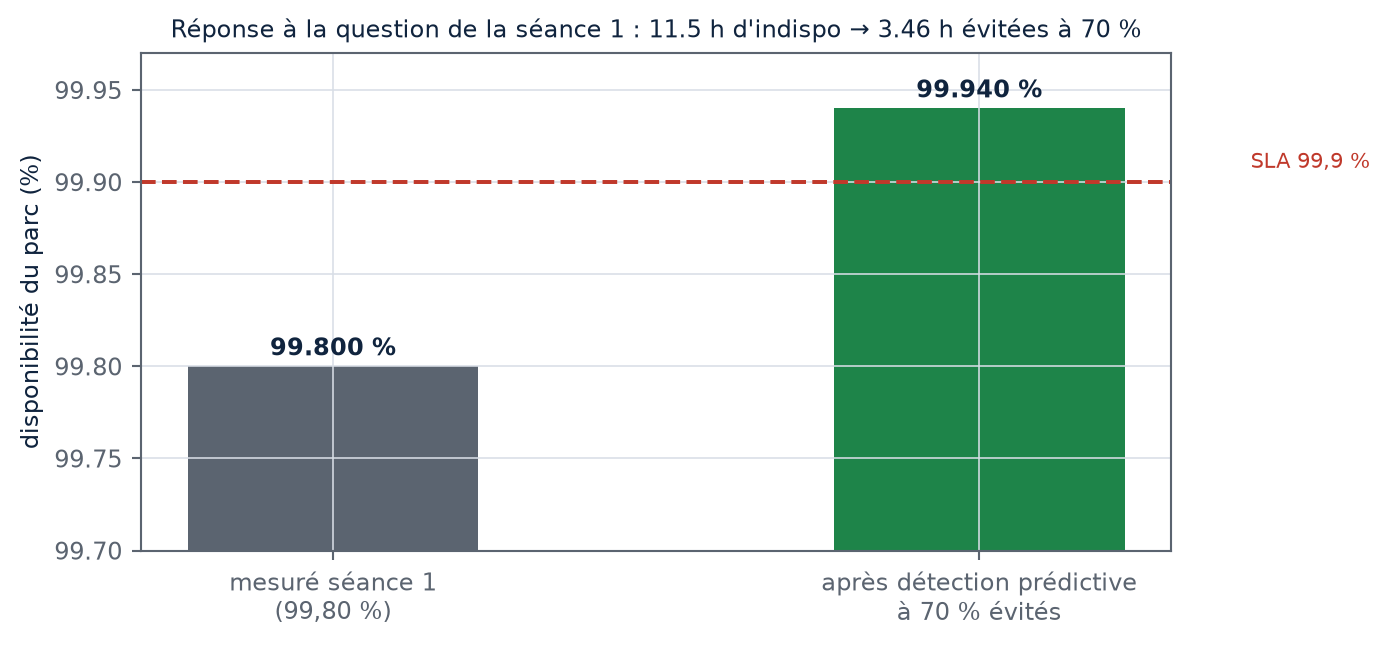
\includegraphics[width=\textwidth]{f24_dispo_predictif.png}
\end{center}
\begin{kbox}[La boucle est bouclée]
Le rappel du détecteur EST un chiffre d'ingénierie de dispo :
passer de 0 à 0,625 de rappel, c'est racheter plus de la moitié
de l'indisponibilité. La séance 4 prolonge : \textbf{prédire}
quand, pas seulement \emph{si}.
\end{kbox}
\end{column}
\end{columns}
\end{frame}

\begin{frame}{À retenir de la séance 3}
\footnotesize%
\begin{columns}[t]
\begin{column}{0.48\textwidth}
\begin{kbox}[Les 5 idées à emporter]
\begin{enumerate}
\item \textbf{Anomalie $\ne$ incident} : le non-supervisé
(IsolationForest, LOF) name le soupçon ; le supervisé décide.
\item À 0,35 \% de positifs, \textbf{l'exactitude ne veut
rien dire} (99,65 \% en ne prédisant jamais 1).
\item \textbf{Précision/rappel/F1} et courbe PR --- jamais la
ROC --- disent la vérité métier.
\item Le \textbf{seuil est un choix métier} : budget NOC,
coût FP (fatigue) vs FN (SLA).
\item \textbf{Validation temporelle obligatoire}
(\py{TimeSeriesSplit}) : KFold mélangé $=$ fuite.
\end{enumerate}
\end{kbox}
\end{column}
\begin{column}{0.48\textwidth}
\begin{block}{Le palmarès mesuré du jour (test, corrigé)}
\begin{center}\small
\begin{tabular}{@{}l c c@{}}
\toprule
 & $F_1$ & AP\\
\midrule
Gradient boosting & \textbf{0,769} & \textbf{0,63}\\
Reg. logistique & 0,12 & 0,32\\
Forêt (balanced, seuil 0,5) & 0,00 & 0,19\\
\bottomrule
\end{tabular}
\end{center}
\end{block}
\begin{wbox}[Et le rappel manquant ?]
24 incidents sur 64 non détectés au seuil optimal. Piste de la
séance 4 : prédire la trajectoire (SARIMA) et agir \emph{avant}.
\end{wbox}
\end{column}
\end{columns}
\end{frame}

\begin{frame}{Prochaine séance --- Séance 4}
\begin{columns}[t]
\begin{column}{0.48\textwidth}
\begin{kbox}[Séries temporelles et prédiction]
\begin{itemize}
\item \textbf{SARIMA} : tendance, saisonnalité journalière et
hebdomadaire de nos métriques (les \py{h\_sin}/\py{js\_sin} du
TP2 étaient la version artisanale).
\item \textbf{Prédiction de panne} : de « cette fenêtre est
anormale » à « ce serveur tombera dans N heures ».
\item \textbf{Capacité} : extrapoler la charge et dimensionner
avant la saturation.
\end{itemize}
\end{kbox}
\end{column}
\begin{column}{0.48\textwidth}
\begin{ebox}[À préparer]
\begin{itemize}
\item Rendre le TP de la séance 3 (barème : frame précédente).
\item Relire les séries de \file{nosys\_metriques.csv} :
tendance hebdo, pics de journée --- matière brute du SARIMA.
\item Gardez vos matrices de confusion : nous comparerons
« détecter » (séance 3) et « prédire » (séance 4).
\end{itemize}
\end{ebox}
\end{column}
\end{columns}
\vspace{2mm}
\begin{center}\small
\textbf{Fin de la séance 3} --- vous savez désormais faire
parler un modèle sur des données réelles, sous contrainte métier.
\end{center}
\end{frame}
